\subthesischapter{Definición de los casos de uso}
\subsubthesischapter{Identificación de los actores}
Los actores no son parte del sistema, pero sí pueden intercambiar información con él, ellos representan los roles que juegan una o varias personas, un equipo o un sistema automatizado. La Tabla \ref{tab: actores} muestra los actores identificados en la aplicación de juego serio:

\begin{table}[ht]
    \centering
    \begin{tabularx}{\textwidth}{|l|X|}
        \hline
        \textbf{Actores} & \textbf{Descripción} \\\hline
        Usuario & Individuo que interactúa con el sistema para hacer uso de una rutina de entrenamiento
        como medio de rehabilitación, diversión o entrenamiento físico. \\\hline
        Sistema & Es la misma aplicación que en determinadas ocasiones ejecuta funcionalidades automáticamente producto de la interacción con el pedal motorizado. \\\hline
    \end{tabularx}
    \caption{Descripción de actores.}
    \label{tab: actores}
\end{table}

\subsubthesischapter{Identificación de los casos de usos}    
Cada forma en que los actores usan el sistema se representa con un caso de uso, como fragmentos de funcionalidad que el sistema ofrece para aportar solución a la necesidad de esta aplicación. Los casos de uso que se definen para el sistema propuesto están reflejados en la Tabla \ref{tab: rf} con su respectivo diagrama en las Figuras \ref{fig: use-cases-user} y \ref{fig: use-cases-system}.

\begin{figure}[!ht]
    \centering
    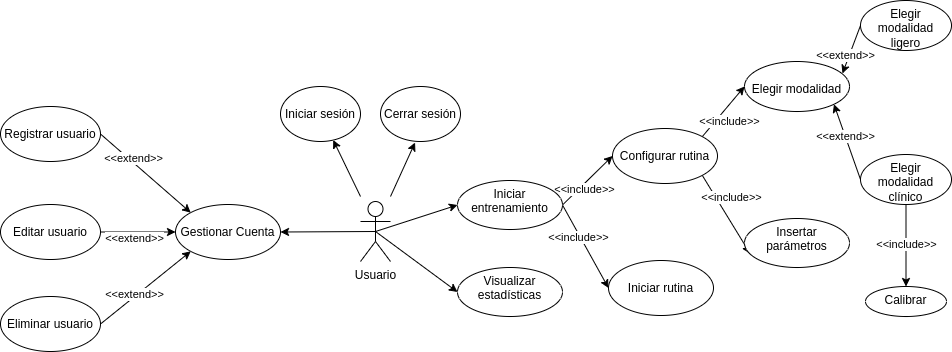
\includegraphics[scale=0.46]{images/diagram-usecase-user.png}
    \caption{Diagrama de casos de uso, actor usuario.}
    \label{fig: use-cases-user}
\end{figure}

\begin{figure}[!ht]
    \centering
    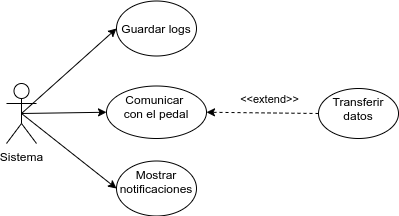
\includegraphics[scale=0.5]{images/diagram-usecase-system.png}
    \caption{Diagrama de casos de uso, actor sistema.}
    \label{fig: use-cases-system}
\end{figure}

\begin{table}[!ht]
>>>>>>> 6987466 (Fixed some tables spaces)
    \centering
    \begin{tabularx}{\textwidth}{|c|X|c|}
        \hline
        \textbf{Casos de uso} & \textbf{Descripción} & \textbf{Requisitos}\\\hline
        Iniciar sesión & Permite al usuario acceder al sistema & RF1\\\hline
        Cerrar sesión & Permite al usuario cerrar sesión en el sistema & RF2\\\hline
        Registrar usuario & Permite guardar los datos de un usuario en la base de datos & RF3\\\hline
        Eliminar usuario & Permite eliminar la cuenta de un usuario en la base de datos & RF4\\\hline
        Editar datos del usuario & Permite actualizar los datos del usuario en la base de datos & RF5\\\hline
        Gestionar cuenta  & Se extiende de los casos de uso registrar usuario, eliminar usuario y editar datos del usuario & RF3, RF4, RF5 \\\hline
        Transferir datos & Permite enviar o recibir datos entre el juego serio y el pedal motorizado & RF6, RF7\\\hline
        Comunicar con pedal & Permite establecer la comunicación entre el juego serio y el pedal motorizado & RF8, RF9\\\hline
        Configurar rutina & Permite elegir la modalidad e insertar los parámetros de la rutina  & RF10\\\hline
        Iniciar rutina & Permite dar inicio a la rutina de entrenamiento & RF11\\\hline
        Pausar/Reanudar rutina & Permite pausar la etapa actual de la rutina & RF12\\\hline
        Finalizar rutina & Permite dar fin a la rutina de entrenamiento & RF13\\\hline
        Entrenar & Se extiende de los casos de uso  iniciar rutina, pausar/reanudar rutina, finalizar rutina&RF11,RF12,RF13\\\hline
        Mostrar rutina & Permite visualizar una rutina de entrenamiento configurada anteriormente &RF14\\\hline
        Visualizar estadística & Permite mostrar estadísticas de las rutinas & RF15\\\hline
        Calibrar sistema & Permite iniciar la calibración para la modalidad clínica  & RF16\\\hline
        Guardar logs & Permite almacenar los hechos ocurridos en el sistema & RF17\\\hline
        Mostrar notificaciones & Permite notificar sobre cualquier error en la aplicación & RF18\\\hline
        %Iniciar juego rutina libre & Permite dar inicio a la rutina de entrenamiento libre \\\hline
        %Iniciar juego rutina resistido & Permite dar inicio a la rutina de entrenamiento resistido \\\hline
    \end{tabularx}
    \caption{Casos de uso del sistema.}
    \label{tab: rf}
\end{table}

\newpage


